% Options for packages loaded elsewhere
\PassOptionsToPackage{unicode}{hyperref}
\PassOptionsToPackage{hyphens}{url}
%
\documentclass[
  russian,
  ignorenonframetext,
]{beamer}
\usepackage{pgfpages}
\usepackage{animate}
\setbeamertemplate{caption}[numbered]
\setbeamertemplate{caption label separator}{: }
\setbeamercolor{caption name}{fg=normal text.fg}
\beamertemplatenavigationsymbolsempty
% Prevent slide breaks in the middle of a paragraph
\widowpenalties 1 10000
\raggedbottom
\setbeamertemplate{part page}{
  \centering
  \begin{beamercolorbox}[sep=16pt,center]{part title}
    \usebeamerfont{part title}\insertpart\par
  \end{beamercolorbox}
}
\setbeamertemplate{section page}{
  \centering
  \begin{beamercolorbox}[sep=12pt,center]{part title}
    \usebeamerfont{section title}\insertsection\par
  \end{beamercolorbox}
}
\setbeamertemplate{subsection page}{
  \centering
  \begin{beamercolorbox}[sep=8pt,center]{part title}
    \usebeamerfont{subsection title}\insertsubsection\par
  \end{beamercolorbox}
}
\AtBeginPart{
  \frame{\partpage}
}
\AtBeginSection{
  \ifbibliography
  \else
    \frame{\sectionpage}
  \fi
}
\AtBeginSubsection{
  \frame{\subsectionpage}
}
\usepackage{lmodern}
\usepackage{amssymb,amsmath}
\usepackage{ifxetex,ifluatex}
\ifnum 0\ifxetex 1\fi\ifluatex 1\fi=0 % if pdftex
  \usepackage[T1]{fontenc}
  \usepackage[utf8]{inputenc}
  \usepackage{textcomp} % provide euro and other symbols
\else % if luatex or xetex
  \usepackage{unicode-math}
  \defaultfontfeatures{Scale=MatchLowercase}
  \defaultfontfeatures[\rmfamily]{Ligatures=TeX,Scale=1}
\fi
\usetheme[subsectionpage=simple,numbering=fraction,progressbar=frametitle,block=fill]{metropolis}
\usefonttheme{professionalfonts}
% Use upquote if available, for straight quotes in verbatim environments
\IfFileExists{upquote.sty}{\usepackage{upquote}}{}
\IfFileExists{microtype.sty}{% use microtype if available
  \usepackage[]{microtype}
  \UseMicrotypeSet[protrusion]{basicmath} % disable protrusion for tt fonts
}{}
\makeatletter
\@ifundefined{KOMAClassName}{% if non-KOMA class
  \IfFileExists{parskip.sty}{%
    \usepackage{parskip}
  }{% else
    \setlength{\parindent}{0pt}
    \setlength{\parskip}{6pt plus 2pt minus 1pt}}
}{% if KOMA class
  \KOMAoptions{parskip=half}}
\makeatother
\usepackage{xcolor}
\IfFileExists{xurl.sty}{\usepackage{xurl}}{} % add URL line breaks if available
\IfFileExists{bookmark.sty}{\usepackage{bookmark}}{\usepackage{hyperref}}
\hypersetup{
  pdftitle={Байесовская оптимизации для вывода демографических историй},
  pdfauthor={Илья Шешуков},
  hidelinks,
  pdfcreator={LaTeX via pandoc}}
\urlstyle{same} % disable monospaced font for URLs
\newif\ifbibliography
\usepackage{graphicx,grffile}
\makeatletter
\def\maxwidth{\ifdim\Gin@nat@width>\linewidth\linewidth\else\Gin@nat@width\fi}
\def\maxheight{\ifdim\Gin@nat@height>\textheight\textheight\else\Gin@nat@height\fi}
\makeatother
% Scale images if necessary, so that they will not overflow the page
% margins by default, and it is still possible to overwrite the defaults
% using explicit options in \includegraphics[width, height, ...]{}
\setkeys{Gin}{width=\maxwidth,height=\maxheight,keepaspectratio}
% Set default figure placement to htbp
\makeatletter
\def\fps@figure{htbp}
\makeatother
\usepackage[normalem]{ulem}
% Avoid problems with \sout in headers with hyperref
\pdfstringdefDisableCommands{\renewcommand{\sout}{}}
\setlength{\emergencystretch}{3em} % prevent overfull lines
\providecommand{\tightlist}{%
  \setlength{\itemsep}{0pt}\setlength{\parskip}{0pt}}
\setcounter{secnumdepth}{-\maxdimen} % remove section numbering
\usepackage{xcolor}
\usepackage{xspace}
\newcommand{\dadi}{∂a∂i\ }
\usepackage{unicode-math}
\usepackage{booktabs}
\ifxetex
  % Load polyglossia as late as possible: uses bidi with RTL langages (e.g. Hebrew, Arabic)
  \usepackage{polyglossia}
  \setmainlanguage[]{russian}
\else
  \usepackage[shorthands=off,main=russian]{babel}
\fi

\title{Байесовская оптимизации для вывода демографических историй}
\author[Илья Шешуков]{Илья Шешуков (СПбГУ)\\[10mm]{\small Руководители: Екатерина Носкова (Университет ИТМО) \\ \phantom{Руководители:} Вячеслав Боровицкий (СПбГУ, ПОМИ РАН) }}
\date{}

\begin{document}
\frame{\titlepage}

\hypertarget{ux432ux432ux435ux434ux435ux43dux438ux435}{%
\section{Введение}\label{ux432ux432ux435ux434ux435ux43dux438ux435}}

\begin{frame}{Демографическая модель популяции}
\protect\hypertarget{ux434ux435ux43cux43eux433ux440ux430ux444ux438ux447ux435ux441ux43aux430ux44f-ux43cux43eux434ux435ux43bux44c-ux43fux43eux43fux443ux43bux44fux446ux438ux438}{}

Имея геномы людей, хотим понять как изменялись их популяции. Как
менялась численность, когда популяции разделялись, как сильно они
мигрировали.

\begin{figure}
\centering
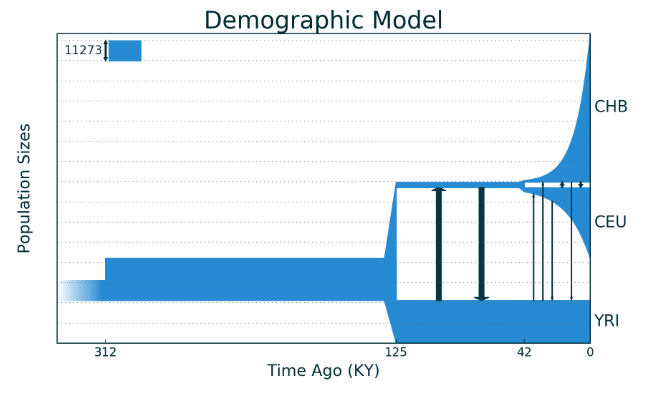
\includegraphics[width=\textwidth,height=0.4\textheight]{./pics/outofafrica.png}
\caption{Демографическая модель африканского происхождени человека}
\end{figure}

\end{frame}

\begin{frame}{Аллель-частотный спектр}
\protect\hypertarget{ux430ux43bux43bux435ux43bux44c-ux447ux430ux441ux442ux43eux442ux43dux44bux439-ux441ux43fux435ux43aux442ux440-1}{}

Аллель-частотный спектр это распределение частоты аллелей в данных
локусах в популяции или выборке.

\begin{figure}
\centering
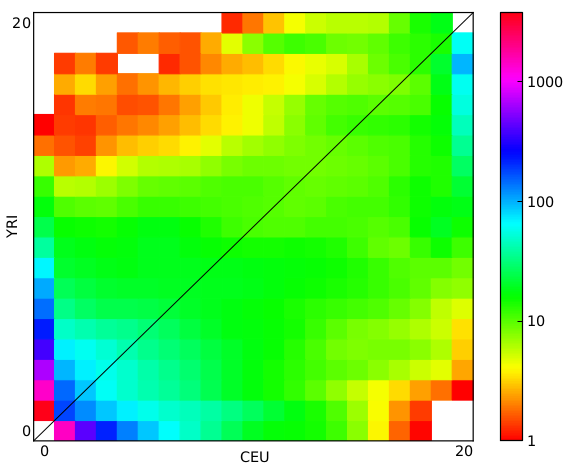
\includegraphics[width=0.5\textwidth,height=\textheight]{./pics/sfs.png}
\caption{График АЧС}
\end{figure}

\end{frame}

\hypertarget{ux43aux430ux43a-ux44dux442ux43e-ux434ux435ux43bux430ux435ux442ux441ux44f-ux441ux435ux439ux447ux430ux441}{%
\section{Как это делается
сейчас}\label{ux43aux430ux43a-ux44dux442ux43e-ux434ux435ux43bux430ux435ux442ux441ux44f-ux441ux435ux439ux447ux430ux441}}

\begin{frame}{∂a∂i\ }
\protect\hypertarget{section}{}

\url{https://bitbucket.org/gutenkunstlab/dadi/}

\begin{itemize}
\tightlist
\item
  Плюсы

  \begin{itemize}
  \tightlist
  \item
    Она работает
  \item
    Ей пользуются реальные люди
  \end{itemize}
\item
  Минусы

  \begin{itemize}
  \tightlist
  \item
    Решает дифференциальное уравнение в частных производных, что долго
  \item
    Использует методы локальной оптимизации, что малоэффективно
  \item
    Для работы необходимо руками писать Питон
  \end{itemize}
\end{itemize}

\end{frame}

\begin{frame}{moments}
\protect\hypertarget{moments}{}

\url{https://bitbucket.org/simongravel/moments}

\begin{itemize}
\tightlist
\item
  Плюсы

  \begin{itemize}
  \tightlist
  \item
    Эффективнее, чем ∂a∂i\ , особенно на больших популяциях
  \end{itemize}
\end{itemize}

\end{frame}

\begin{frame}{GADMA}
\protect\hypertarget{gadma}{}

\url{https://github.com/ctlab/GADMA}

\begin{itemize}
\tightlist
\item
  Основана на ∂a∂i\ и moments
\item
  Использует генетический алгоритм для поиска значения параметров
  демографической модели
\item
  Не требует человеческого вмешательства
\end{itemize}

\end{frame}

\begin{frame}[standout]{Что можно сделать}
\protect\hypertarget{ux447ux442ux43e-ux43cux43eux436ux43dux43e-ux441ux434ux435ux43bux430ux442ux44c}{}

Заменим генетический алгоритм байесовской оптимизацей.

\end{frame}

\begin{frame}{Байесовская оптимизация}
\protect\hypertarget{ux431ux430ux439ux435ux441ux43eux432ux441ux43aux430ux44f-ux43eux43fux442ux438ux43cux438ux437ux430ux446ux438ux44f}{}

\begin{itemize}
\tightlist
\item
  Алгоритм глобальной оптимизации
\item
  Хорошо работает для сложновычислимых функций (например, если нужно
  решать уравнение в частных производных), т.е. хорошо подходит для
  задачи
\item
  Можно параллелить
\item
  Менее эвристична, чем генетический алгоритм
\end{itemize}

\end{frame}

\begin{frame}{Красивые графики работы GPyOpt}
\protect\hypertarget{ux43aux440ux430ux441ux438ux432ux44bux435-ux433ux440ux430ux444ux438ux43aux438-ux440ux430ux431ux43eux442ux44b-gpyopt}{}

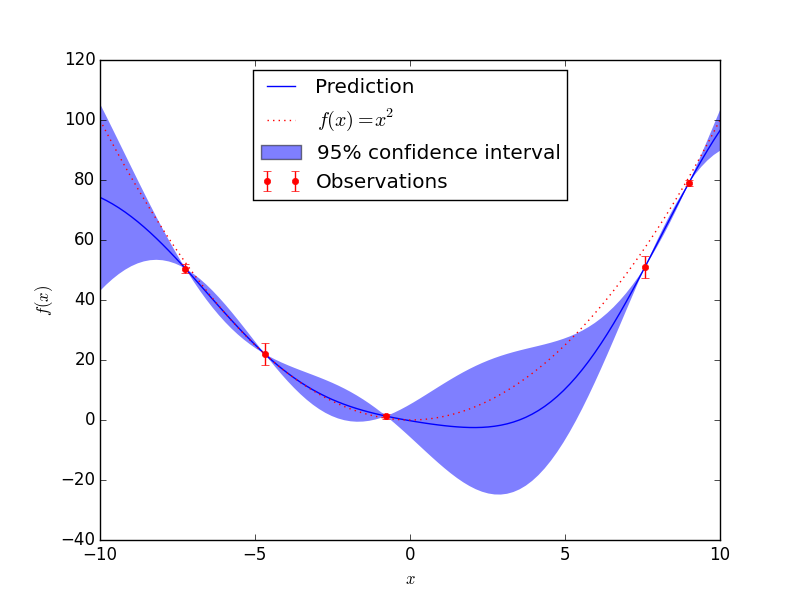
\includegraphics[width=0.4\textwidth,height=\textheight]{./pics/bayes.png}
~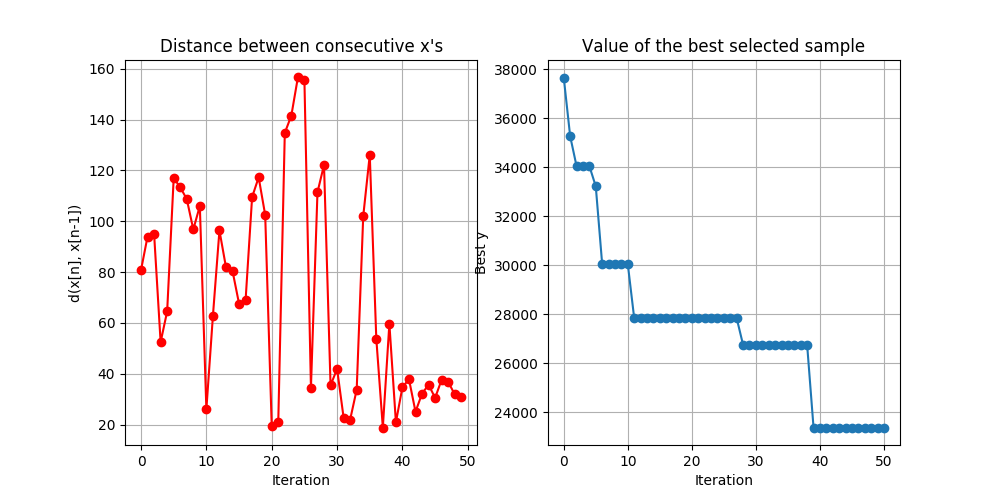
\includegraphics[width=0.5\textwidth,height=\textheight]{./pics/conv.png}

\end{frame}

\begin{frame}{Красивые графики работы GPyOpt}
  \animategraphics[autoplay,loop,width=\linewidth]{2}{anim/}{1}{17}
\end{frame}

\hypertarget{ux440ux435ux437ux443ux43bux44cux442ux430ux442ux44b}{%
\section{Результаты}\label{ux440ux435ux437ux443ux43bux44cux442ux430ux442ux44b}}

\begin{frame}{Планы (промежуточная презентация)}
\protect\hypertarget{ux43fux43bux430ux43dux44b-ux43fux440ux43eux43cux435ux436ux443ux442ux43eux447ux43dux430ux44f-ux43fux440ux435ux437ux435ux43dux442ux430ux446ux438ux44f}{}

\begin{itemize}
\tightlist
\item
  Заменить в ∂a∂i\ алгоритм градиентного спуска нa байесовскую
  оптимизацию.
\item
  Посмотреть станет ли лучше
\item
  Интегрировать в GADMA
\end{itemize}

\end{frame}

\begin{frame}{Реальность}
\protect\hypertarget{ux440ux435ux430ux43bux44cux43dux43eux441ux442ux44c}{}

\begin{itemize}
\tightlist
\item[$\boxtimes$]
  Заменить в \sout{∂a∂i\ } moments алгоритм градиентного спуска нa
  байесовскую оптимизацию.
\item[$\boxtimes$]
  Посмотреть станет ли лучше
\item[$\square$]
  Интегрировать в GADMA
\end{itemize}

\end{frame}

\begin{frame}{Что мы делали}
\protect\hypertarget{ux447ux442ux43e-ux43cux44b-ux434ux435ux43bux430ux43bux438}{}

\begin{itemize}
\tightlist
\item
  Копались в библиотеках
\item
  Нашли баги в GPyOpt
\item
  Играли с гиперпараметрами
\item
  Думали, почему всё работает плохо
\item
  Очень долго ждали
\end{itemize}

\end{frame}

\begin{frame}{Сравнение}
\protect\hypertarget{ux441ux440ux430ux432ux43dux435ux43dux438ux435}{}

\begin{figure}
\centering
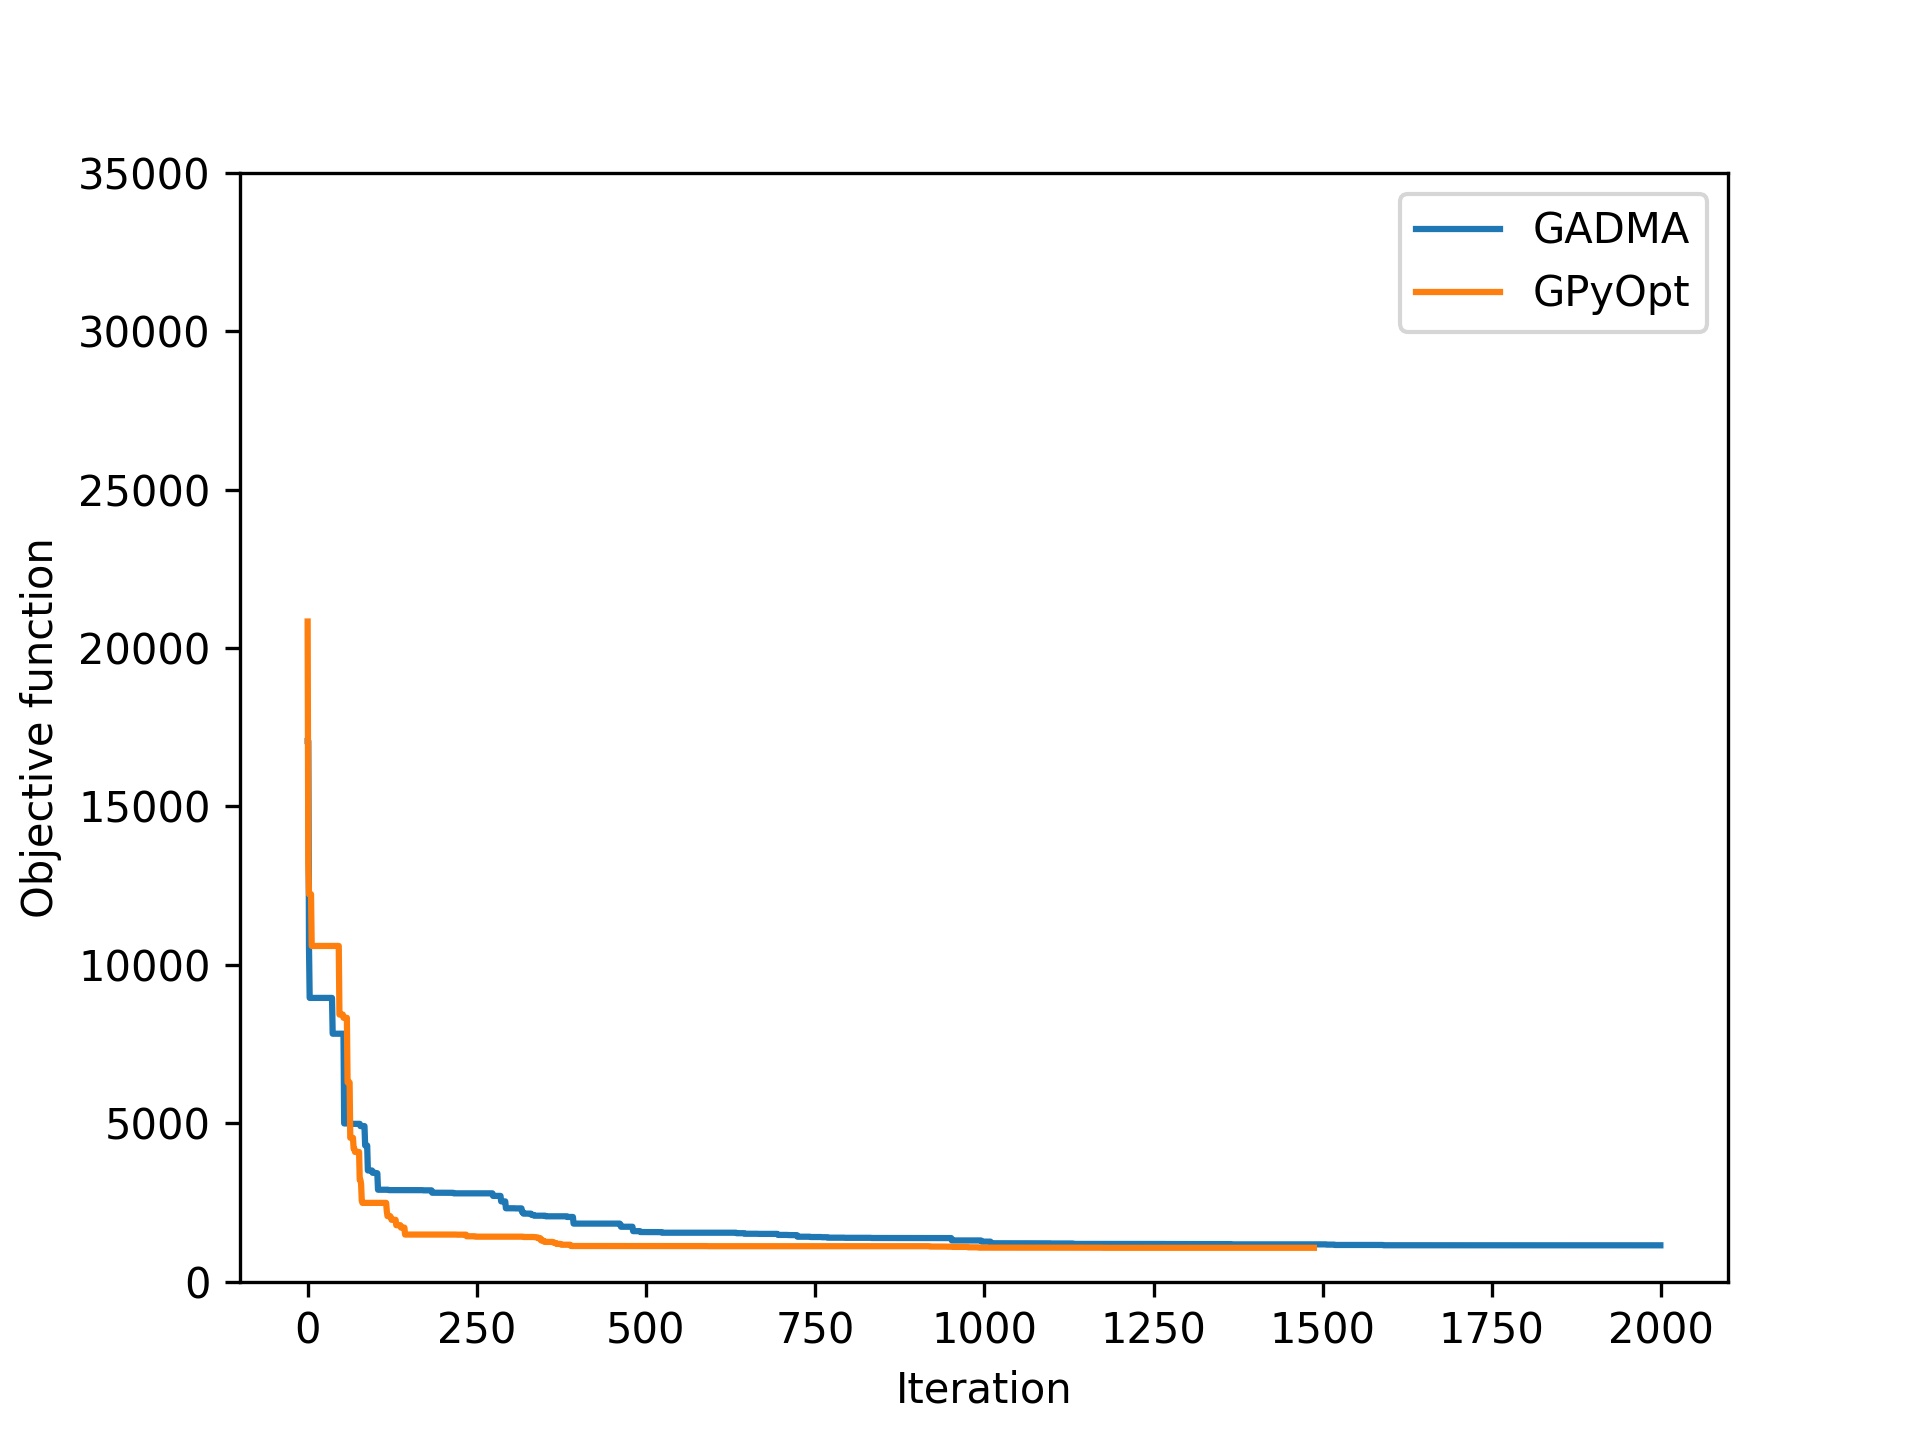
\includegraphics[width=0.8\textwidth,height=\textheight]{./plots/2pop_6.best.log.png}
\caption{2 популяции, 6 переменных}
\end{figure}

\end{frame}

\begin{frame}{Сравнение}
\protect\hypertarget{ux441ux440ux430ux432ux43dux435ux43dux438ux435-1}{}

\begin{figure}
\centering
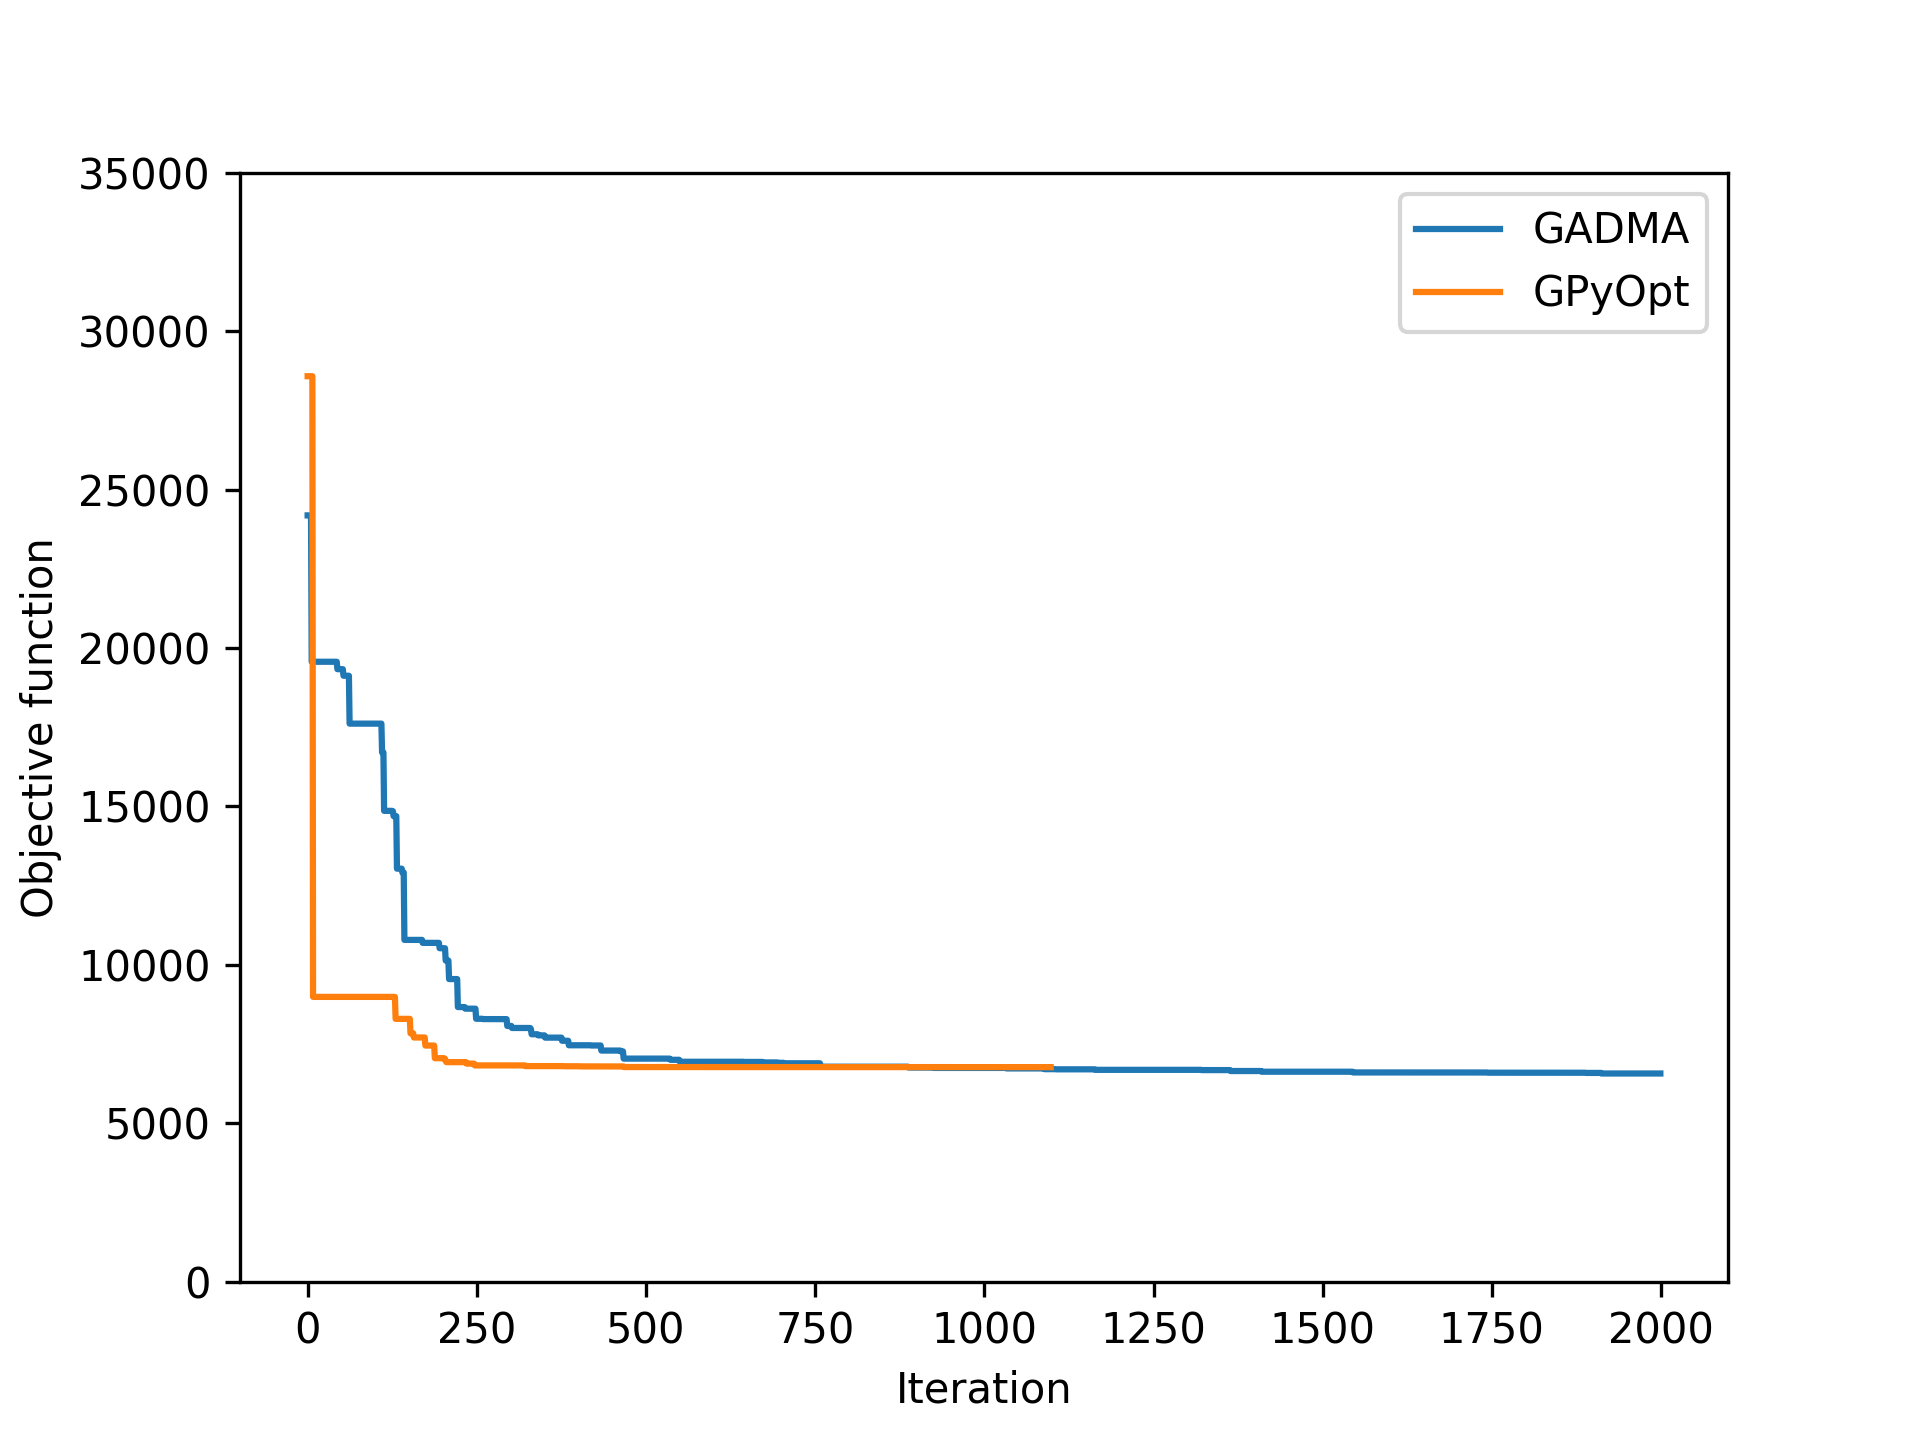
\includegraphics[width=0.8\textwidth,height=\textheight]{./plots/3pop_13.best.log.png}
\caption{3 популяции, 13 переменных}
\end{figure}

\end{frame}

\begin{frame}{Итого}
\protect\hypertarget{ux438ux442ux43eux433ux43e}{}

\begin{itemize}
\tightlist
\item
  Байесовская оптимизация оправдывает себя, особенно если вычисления
  функции очень дорогие (как у ∂a∂i)
\item
  Но всё равно, \alert{пока} работает не так хорошо, как могла бы (т.е.
  лучше всех)
\end{itemize}

\end{frame}

\begin{frame}{Что бы хотелось ещё сделать}
\protect\hypertarget{ux447ux442ux43e-ux431ux44b-ux445ux43eux442ux435ux43bux43eux441ux44c-ux435ux449ux451-ux441ux434ux435ux43bux430ux442ux44c}{}

\begin{itemize}
\tightlist
\item
  Потестировать на других данных
\item
  Потестировать на разных гиперпараметрах; найти такие, которые будут работать лучше всего

\item
  Интегрировать в GADMA
\end{itemize}

\end{frame}

\begin{frame}[standout]{Конец}
\protect\hypertarget{ux43aux43eux43dux435ux446}{}

Спасибо за внимание

\end{frame}

\end{document}
